\documentclass[9pt]{beamer}
\usepackage{silence}
\WarningFilter{beamerthememetropolis}{You need to compile with XeLaTeX or LuaLaTeX to use the Fira fonts}
\usetheme[titleformat = smallcaps, block = fill, progressbar = frametitle]{metropolis}
\title{\Huge Integral Calculus}
%---------------------------------%
% PACKAGES
%---------------------------------%
% Input encoding.
\usepackage[utf8]{inputenc} % For accents in spanish: transforms "á" into "\'a"
\usepackage[T1]{fontenc} % Output encoding. Use to avoid silly problems on the output.
                         % See: http://tex.stackexchange.com/questions/664/why-should-i-use-usepackaget1fontenc
\usepackage[sfdefault]{FiraSans}
\usepackage{FiraMono}
% AMS packages
\usepackage{amsmath}
\usepackage{amsfonts}
\usepackage{amssymb}
\usepackage{amsthm}
% Matrices
\usepackage{mathtools}
\newcommand{\verteq}{\rotatebox{90}{$\,=$}}
\usepackage{gauss}
% Customization for augmented matrices; 
% see https://tex.stackexchange.com/questions/146723/how-to-typeset-row-operations-on-augmented-matrix
% Patch gauss macros for doing their work in `align'
% and other amsmath environments; see http://tex.stackexchange.com/questions/146532/
\usepackage{etoolbox}
\makeatletter
\patchcmd\g@matrix
    {\vbox\bgroup}
    {\vbox\bgroup\normalbaselines} % restore the standard baselineskip
    {}{}
\makeatother
\newcommand{\BAR}{%
    \hspace{-\arraycolsep}%
    \strut\vrule % the `\vrule` is as high and deep as a strut
    \hspace{-\arraycolsep}%
}
% Math blackboard font
\usepackage{bbm}
% Fonts
\usepackage{lmodern} 
% \usepackage[sfdefault]{FiraSans}
\usepackage[normalem]{ulem}
\usepackage{eulervm}
% Graphics
\usepackage{graphicx} 
\usepackage{float}
\usepackage{subcaption}
\usepackage{wrapfig}
\usepackage{animate}
\usepackage{caption}
% Algorithms
\usepackage[ruled]{algorithm2e}
\newcommand{\lIfElse}[3]{\lIf{#1}{#2 \textbf{else}~#3}}
% Boxes
\usepackage[most]{tcolorbox}
% For reference enumerations lists
\usepackage{enumitem}
% \setlist{labelwidth = \widthof{0.}, leftmargin = {\labelwidth+\labelsep}, 
%         rightmargin = \leftmargin} % Setting left marging = right marging in itemize envirnment
% Import icons
\usepackage{fontawesome}
% Hyperlink
\usepackage{hyperref}
\hypersetup{
	final,
    bookmarksnumbered=true,
    bookmarksopen=true,
    bookmarksopenlevel=0,
    unicode=false,          % non-Latin characters in Acrobat?s bookmarks
    pdftoolbar=true,        % show Acrobat?s toolbar?
    pdfmenubar=true,        % show Acrobat?s menu?
    pdffitwindow=false,     % window fit to page when opened
    pdftitle={Introduction to Mathematics},    % title
    pdfdisplaydoctitle=true, %display document title instead of file name in title bar
    pdftoolbar=true,
    pdfmenubar=true,
    pdflang={English},
    pdfauthor={Abel Guada Azze},     % author
    pdfsubject={Introduction to Mathematics},   % subject of the document
    pdfcreator={Abel Guada Azze},   % creator of the document
    pdfproducer={Abel Guada Azze}, % producer of the document
    pdfkeywords={Mathematics} {introduction}, % list of keywords
    pdfnewwindow=true,      % links in new window
    breaklinks=true,
    hidelinks,
    colorlinks,
    linkcolor=black,          % color of internal links (change box color with linkbordercolor)
    citecolor=black,        % color of links to bibliography
    filecolor=cyan,      % color of file links
    urlcolor=magenta           % color of external links
}
%----------------------------------- Tikz
\usepackage{tikz}
\usepackage{pgfplots}
% \pgfplotsset{compat=1.18}
% \usepackage{tkz-euclide}
\usetikzlibrary{shapes,arrows.meta,matrix,positioning,calc}
\newcommand{\tikzmark}[1]{\tikz[baseline,remember picture] \coordinate (#1) {};}
% ---------- Helpers: 2-set and 3-set Venns ----------
% \VennTwoCounts{LabelA}{LabelB}{onlyA}{both}{onlyB}{Neither}{Universe}
\newcommand{\VennTwoCounts}[7]{%
  \begin{tikzpicture}[scale=1.0,baseline=(current bounding box.center)]
    \def\r{1.8}   % circle radius (cm)
    \def\dx{2.35} % distance between centres (cm)
    \def\pad{0.60} % padding between circles and rectangle (cm)

    \coordinate (A) at (0,0);
    \coordinate (B) at (\dx,0);

    % Universe rectangle (outline only)
    \draw[line width=.8pt, rounded corners=2pt]
      ($(A)+(-\r-\pad,-\r-\pad)$) rectangle ($(B)+(\r+\pad,\r+\pad)$);

    % Set fills + outlines
    \fill[black!8] (A) circle (\r);
    \fill[black!8] (B) circle (\r);
    \draw[line width=.8pt] (A) circle (\r);
    \draw[line width=.8pt] (B) circle (\r);

    % Universe label (top-left inside the box)
    \node[font=\scriptsize,anchor=north west]
      at ($(A)+(-\r-\pad+0.12,\r+\pad-0.12)$) {#7};

    % Set labels
    \node[font=\small\bfseries] at ($(A)+(0,0.68*\r)$) {#1};
    \node[font=\small\bfseries] at ($(B)+(0,0.68*\r)$) {#2};

    % Counts
    \node[font=\small] at ($ (A)+(-0.60*\r,-0.05*\r) $) {#3}; % only A
    \node[font=\small] at ($ .5*(A)+.5*(B) $) {#4};           % both
    \node[font=\small] at ($ (B)+(0.60*\r,-0.05*\r) $) {#5};  % only B
    \node[font=\small]
      at ($ (B)+(\r+0.3*\pad,0.78*\r) $) {#6};                % outside
  \end{tikzpicture}%
}


%---------------------------------%
% Biblio
%---------------------------------%

%---------------------------------%
% SETTINGS
%---------------------------------%
% displays sections and subsections numbered in the TOC
\setbeamertemplate{section in toc}[sections numbered]
% \setbeamertemplate{subsection in toc}[subsections numbered]
% gets rid of bottom navigation bars
\setbeamertemplate{footline}{}
% gets rid of bottom navigation symbols
\setbeamertemplate{navigation symbols}{}
% sets images' path
\graphicspath{{img/}}
% resets footnote counter at the beginning of each section
\AtBeginEnvironment{frame}{\setcounter{footnote}{0}}
% beamer margins
\setbeamersize
{
    text margin left=3mm,
    text margin right=3mm,
    % sidebar width left=.0cm,
    % sidebar width right=.0cm,
    % description width,
    % description width of=,
    % mini frame size=,
    % mini frame offset
}
% redefines block environment to add small space between title and content
\let\oldblock\block
\let\endoldblock\endblock
\renewenvironment{block}[1]
    {\begin{oldblock}{#1}
        \vspace{0.1cm}
    }
    { 
    \end{oldblock}
    }

%---------------------------------%
% SETTINGS
%---------------------------------%
%---------------------------------%
% TITLE PAGE
%---------------------------------%
\setbeamertemplate{title page}{
    \vspace{-0.4cm}
    
    \textcolor{CUNEForange}{\rule{\textwidth}{0.05cm}}
    \vspace{-0.65cm}
    
    \begin{minipage}{0.2\textwidth}
        \includegraphics[width = 2.0cm]{Logo-CUNEF.png}
    \end{minipage}
    \begin{minipage}{0.7\textwidth}
        
        \quad \Huge \usebeamertemplate*{title}
        
    \end{minipage}    
    \vspace{-0.25cm}
    
    \textcolor{CUNEForange}{\rule{\textwidth}{0.05cm}}
    \vspace{1.5cm}

    \begin{minipage}{0.075\textwidth}
        
    \end{minipage}\hfill\textcolor{CUNEForange}{\vrule\vrule\vrule}
    \begin{minipage}{0.825\textwidth}
        \begin{itemize}[leftmargin = *, label= $ $]
            \item {\hspace{1.05pt} \faUser\quad Abel Guada Azze}
            \item {\hspace{0pt} \faEnvelope\quad \href{mailto:abel.guada@cunef.edu}{abel.guada@cunef.edu}}
            \item {\hspace{0pt} \faSuitcase\quad F4.5 - C. de Leonardo Prieto Castro, 2}
            \item {\hspace{0pt} \faUniversity\ \ \ Department of Quantitative Methods - CUNEF Universidad}
            \item {\hspace{0pt} \faGraduationCap\ \ \ Bachelor in Philosophy, Politics and Economics}
        \end{itemize}
    \end{minipage}
}
\setbeamertemplate{title}{
  \linespread{1.0}%
  \inserttitle%
  \par%
  \vspace*{0.5em}
}
\setbeamertemplate{subtitle}{
  \insertsubtitle%
  \par%
  \vspace*{0.5em}
}
\titlegraphic{
\includegraphics[height = 2.0cm]{logo-CUNEF.png}}	
\author[]{Abel G. Azze}
\institute[]{Department of Quantitative Methods \\ CUNEF Universidad}
\date{}
%---------------------------------%
% TITLE PAGE
%---------------------------------%
%---------------------------------%
% CUSTOM COMMANDS AND DEFINITIONS
%---------------------------------%
% define new colors
\definecolor{amber}{rgb}{1.0, 0.49, 0.0}
\definecolor{firebrick3}{RGB}{207, 33, 32}
\definecolor{deepskyblue3}{RGB}{0, 155, 206}
\definecolor{darkorange3}{RGB}{206, 102, 0}
\definecolor{darkolivegreen3}{RGB}{163, 207, 91}
\definecolor{CUNEForange}{RGB}{237, 114, 1}
\definecolor{CUNEFblue}{RGB}{36, 51, 71}
\definecolor{background-gray}{RGB}{251, 251, 250}
\definecolor{block-background-gray}{RGB}{229, 230, 230}
% coloring commands
\newcommand{\red}[1]{\textcolor{firebrick3}{#1}}
\newcommand{\black}[1]{\textcolor{black}{#1}}
\newcommand{\blue}[1]{\textcolor{deepskyblue3}{#1}}
\newcommand{\green}[1]{\textcolor{darkolivegreen3}{#1}}
\newcommand{\orange}[1]{\textcolor{darkorange3}{#1}}
\newcommand{\purple}[1]{\textcolor{purple}{#1}}
\newcommand{\Corange}[1]{\textcolor{CUNEForange}{#1}}
\newcommand{\Cblue}[1]{\textcolor{CUNEFblue}{#1}}
% footnote without number
\newcommand\footnotenonum[1]{%
  \begingroup
  \renewcommand\thefootnote{}\footnote{#1}%
  \addtocounter{footnote}{-1}%
  \endgroup
}
% hyperbolic secant
\DeclareMathOperator{\sech}{sech}
\DeclareMathOperator{\csch}{csch}
% Plain macros
\newcommand{\N}{\mathbb{N}} % natural number set
\newcommand{\Z}{\mathbb{Z}} % entire number set
\newcommand{\Q}{\mathbb{Q}} % rational number set
\newcommand{\R}{\mathbb{R}} % real number set
\newcommand{\I}{\mathbb{I}} % imaginary number set
\newcommand{\cF}{\mathcal{F}} % sigma-algebra
\newcommand{\cD}{\mathcal{D}} % stopping set
\newcommand{\cX}{\mathcal{X}} % bridge sets
\newcommand{\cC}{\mathcal{C}} % continuation set
\newcommand{\cB}{\mathcal{B}} % ball around a point
\newcommand{\cA}{\mathcal{A}} % subset of R+xR
\newcommand{\cR}{\mathcal{R}} % compact set
\newcommand{\cN}{\mathcal{N}} % normal distribution
\newcommand{\rmd}{\mathrm{d}} % differential operator
\newcommand{\rmb}{\mathsf{b}} % OSB of the original OSP
\newcommand{\rK}{\mathsf{K}} % Kernel of the original OSP
\newcommand{\rPhi}{\mathsf{\Phi}} % Phi of the original OSP
\newcommand{\rphi}{\mathsf{\boldsymbol{\phi}}} % Phi of the original OSP
\newcommand{\InfGen}{\mathbb{L}} % infinitesimal generator
\newcommand{\InfGenOr}{\mathsf{L}} % infinitesimal generator. Original version
\newcommand{\Ind}{\mathbbm{1}} % indicator function
\newcommand{\lp}{\left(} % left parenthesis
\newcommand{\rp}{\right)} % right parenthesis
\newcommand{\lb}{\left[} % left brackets
\newcommand{\rb}{\right]} % right brackets
\newcommand{\lc}{\left\{} % left curly brackets
\newcommand{\rc}{\right\}} % right curly brackets
\newcommand{\blp}{\big(}
\newcommand{\brp}{\big)}
\newcommand{\blb}{\big[}
\newcommand{\brb}{\big]}
\newcommand{\blc}{\big\{}
\newcommand{\brc}{\big\}}
% Macros with arguments
\newcommand\redsout{\bgroup\markoverwith{\textcolor{red}{\rule[0.5ex]{2pt}{0.4pt}}}\ULon}
\newcommand\bluesout{\bgroup\markoverwith{\textcolor{blue}{\rule[0.5ex]{2pt}{0.4pt}}}\ULon}
\newcommand{\lrav}[1]{\left|#1\right|} % absolute value
\newcommand{\wt}[1]{\widetilde{#1}}
\newcommand{\wh}[1]{\widehat{#1}}
\newcommand{\ol}[1]{\overline{#1}}
\newcommand{\ul}[1]{\underline{#1}}
\newcommand{\lrp}[1]{\lp#1\rp} % left-right parenthesis
\newcommand{\lrb}[1]{\lb#1\rb} % left-right brackets
\newcommand{\lrc}[1]{\lc#1\rc} % left-right curly brackets
\newcommand{\blrp}[1]{\blp#1\brp} % big left-right parenthesis
\newcommand{\blrb}[1]{\blb#1\brb} % big left-right brackets
\newcommand{\blrc}[1]{\blc#1\brc} % big left-right curly brackets
\newcommand{\Prob}[1]{\mathbb{P}\lp #1\rp} % probability 1
\newcommand{\Pro}[2]{\mathbb{P}_{#2}\lp #1\rp} % probability 2
\renewcommand{\Pr}{\mathbb{P}} % probability 3
\newcommand{\PProb}[1]{\mathsf{P}\lp #1\rp} % probability 1.2
\newcommand{\PPro}[2]{\mathsf{P}_{#2}\lp #1\rp} % probability 2.2
\newcommand{\PPr}{\mathsf{P}} % probability 3.2
\newcommand{\Esp}[1]{\mathbb{E}\lb #1\rb} % mean 1
\newcommand{\Espbigg}[1]{\mathbb{E}\bigg[\!#1\bigg]} % mean 1 bigg
\newcommand{\Es}[2]{\mathbb{E}_{#2}\lb #1\rb} % mean 2
\newcommand{\Esbigg}[2]{\mathbb{E}_{#2}\bigg[\!#1\bigg]} % mean 2 bigg
\newcommand{\E}{\mathbb{E}} % mean 3
\newcommand{\EEsp}[1]{\mathsf{E}\lb #1\rb} % mean 1.2
\newcommand{\EEs}[2]{\mathsf{E}_{#2}\lb #1\rb} % mean 2.2
\newcommand{\EE}{\mathsf{E}} % mean 3.2
\newcommand{\V}[1]{\mathbb{V}\mathrm{ar}\lb #1\rb} % variance 1
\newcommand{\Vs}[2]{\mathbb{V}\mathrm{ar}_{#2}\lb #1\rb} % variance 2
\newcommand{\VV}[1]{\mathrm{V}\mathrm{ar}\lb #1\rb} % variance 1 original OSP
\newcommand{\VVs}[2]{\mathrm{V}\mathrm{ar}_{#2}\lb #1\rb} % variance 2 original OSP
\newcommand{\Cov}[2]{\mathbb{C}\mathrm{ov}\lb #1,#2\rb} % covariance
\newcommand{\CCov}[2]{\mathsf{C}\mathrm{ov}\lb #1,#2\rb} % covariance original OSP
%---------------------------------%
% CUSTOM COMMANDS AND DEFINITIONS
%---------------------------------%


%----------------------------- -------------- -----------------------------%
%----------------------------- BEGIN DOCUMENT -----------------------------%
%----------------------------- -------------- -----------------------------%
\begin{document}
% TODO
%----------------------- TITLE -----------------------%
\maketitle
%----------------------- TITLE -----------------------%

%----------------------- SERIES -----------------------%
% \section{Series}
%----------------------- SERIES -----------------------%

%----------------------- INTRODUCTION TO INTEGRAL CALCULUS -----------------------%
\section{Introduction to Integral Calculus}

\begin{frame}{What is integral calculus?}

    \textbf{Integral Calculus:} Studies the \textbf{accumulation of quantities}.
    \vspace{0.3cm}

    Classic examples that we are going to visit are finding the \textbf{area under a curve}, computing the \textbf{consumer surplus}, and calculating the \textbf{Gini index}. 
    \vspace{0.3cm}
    
    Key concepts include \textbf{definite and indefinite integrals}, \textbf{integration techniques}, and the \textbf{Fundamental Theorem of Calculus}.
    
\end{frame}

\begin{frame}{Economic motivation: the total consumption value}

    Suppose that instead of making available $7$ units of a product at once, producers put units on the market one after the other, waiting for consumers to buy every unit before delivering the next one.
    \vspace{0.2cm}
    
    \textbf{Problem:} Once $q = 7$ units have been supplied and bought, how much have consumers spent on that product?

    \textbf{Answer:} The Total Consumption Value (TCV) is $P(7) = p_D(1) + p_D(2) + \dots +  p_D(7)$
    
    \textbf{Visual interpretation:} The value $P(7)$ is the sum of the areas of the colored rectangles
    \vspace{0.2cm}
    
    \begin{minipage}{0.62\textwidth}
        
        {\hspace{0.1cm}
        \begin{tikzpicture}
        
        \begin{axis}[
            width = \textwidth,
            height = 4cm,
            axis lines = middle,
            xmin = 0,
            xmax = 7.5,
            ymin = 0,
            ymax = 250,
            xtick = {1, 2, 3, 4, 5, 6, 7},
            % xticklabels = {$q_0$, $q_2$, $q^*$, $q_1$},
            scaled ticks = false,
            ytick = {\empty},
            % yticklabels = {$p_1$, $p^*$, $p_2$, $p_0$},
            ticklabel style = {font=\scriptsize},
            xlabel = $q$,
            ylabel = $p$,
            axis line style = {
                -latex,
                shorten >= -0.3cm,
                % shorten <=-12.5pt,
            },
            xlabel style={at={(ticklabel* cs:1)}, xshift = 0.2cm, anchor=north west},
            ylabel style={at={(ticklabel* cs:1)}, yshift = 0.2cm, anchor=south west},
        ]

            \addplot[thick, deepskyblue3, samples = 51, smooth, domain = 0:7] {0.9*(x-15)^2};

            \draw[fill=orange!30!white] (0, 0) rectangle ++(100, {0.9*(1-15)^2});
            \draw[fill=orange!30!white] (100, 0) rectangle ++(100, {0.9*(2-15)^2});
            \draw[fill=orange!30!white] (200, 0) rectangle ++(100, {0.9*(3-15)^2});
            \draw[fill=orange!30!white] (300, 0) rectangle ++(100, {0.9*(4-15)^2});
            \draw[fill=orange!30!white] (400, 0) rectangle ++(100, {0.9*(5-15)^2});
            \draw[fill=orange!30!white] (500, 0) rectangle ++(100, {0.9*(6-15)^2});
            \draw[fill=orange!30!white] (600, 0) rectangle ++(100, {0.9*(7-15)^2});

        \end{axis}

        \end{tikzpicture} 
        }    
        
        
    \end{minipage}
    \begin{minipage}{0.33\textwidth}
        \textcolor{darkorange3}{What happens if producers deliver products in batches of $0.5$-units instead?}
    \end{minipage}
    
\end{frame}

\begin{frame}{Economic motivation: the total consumption value}

    \centering
    Let $\Delta q$ be the batch size being delivered by producers and bought by consumers
    \vspace{0.5cm}
    
    {\hspace{0.4cm}
    \begin{minipage}{0.475\textwidth}

        {\scriptsize
        \begin{align*}
            \hspace{-0.7cm} \Delta q = 0.5\ \Rightarrow\ P(7) &= 0.5\sum_{n=1}^{14} p_D(n\Delta q)
        \end{align*}
        }
        \vspace{-1.6cm}
        
        {\hspace{0.3cm}
        \begin{tikzpicture}
        
        \begin{axis}[
            width = \textwidth,
            height = 4cm,
            axis lines = middle,
            xmin = 0,
            xmax = 7.5,
            ymin = 0,
            ymax = 250,
            xtick = {1, 2, 3, 4, 5, 6, 7},
            % xticklabels = {$q_0$, $q_2$, $q^*$, $q_1$},
            scaled ticks = false,
            ytick = {\empty},
            % yticklabels = {$p_1$, $p^*$, $p_2$, $p_0$},
            ticklabel style = {font=\scriptsize},
            xlabel = $q$,
            ylabel = $p$,
            axis line style = {
                -latex,
                shorten >= -0.3cm,
                % shorten <=-12.5pt,
            },
            xlabel style={at={(ticklabel* cs:1)}, xshift = 0.2cm, anchor=north west},
            ylabel style={at={(ticklabel* cs:1)}, yshift = 0.2cm, anchor=south west},
        ]

            \addplot[thick, deepskyblue3, samples = 51, smooth, domain = 0:7] {0.9*(x-15)^2};

            \draw[fill=orange!30!white] (0, 0) rectangle ++(50, {0.9*(0.5-15)^2});
            \draw[fill=orange!30!white] (50, 0) rectangle ++(50, {0.9*(1-15)^2});
            \draw[fill=orange!30!white] (100, 0) rectangle ++(50, {0.9*(1.5-15)^2});
            \draw[fill=orange!30!white] (150, 0) rectangle ++(50, {0.9*(2-15)^2});
            \draw[fill=orange!30!white] (200, 0) rectangle ++(50, {0.9*(2.5-15)^2});
            \draw[fill=orange!30!white] (250, 0) rectangle ++(50, {0.9*(3-15)^2});
            \draw[fill=orange!30!white] (300, 0) rectangle ++(50, {0.9*(3.5-15)^2});

            \draw[fill=orange!30!white] (350, 0) rectangle ++(50, {0.9*(4-15)^2});
            \draw[fill=orange!30!white] (400, 0) rectangle ++(50, {0.9*(4.5-15)^2});
            \draw[fill=orange!30!white] (450, 0) rectangle ++(50, {0.9*(5-15)^2});
            \draw[fill=orange!30!white] (500, 0) rectangle ++(50, {0.9*(5.5-15)^2});
            \draw[fill=orange!30!white] (550, 0) rectangle ++(50, {0.9*(6-15)^2});
            \draw[fill=orange!30!white] (600, 0) rectangle ++(50, {0.9*(6.5-15)^2});
            \draw[fill=orange!30!white] (650, 0) rectangle ++(50, {0.9*(7-15)^2});

        \end{axis}

        \end{tikzpicture} 
        }    
        
    \end{minipage}
    \begin{minipage}{0.475\textwidth}
        
        {\scriptsize
        \begin{align*}
            \hspace{-0.9cm} \Delta q = 0.25\ \Rightarrow\ P(7) = 0.25\sum_{n=1}^{28} p_D(n\Delta q)
        \end{align*}
        }
        \vspace{-1.6cm}
        
        {\hspace{0.1cm}
        \begin{tikzpicture}
        
        \begin{axis}[
            width = \textwidth,
            height = 4cm,
            axis lines = middle,
            xmin = 0,
            xmax = 7.5,
            ymin = 0,
            ymax = 250,
            xtick = {1, 2, 3, 4, 5, 6, 7},
            % xticklabels = {$q_0$, $q_2$, $q^*$, $q_1$},
            scaled ticks = false,
            ytick = {\empty},
            % yticklabels = {$p_1$, $p^*$, $p_2$, $p_0$},
            ticklabel style = {font=\scriptsize},
            xlabel = $q$,
            ylabel = $p$,
            axis line style = {
                -latex,
                shorten >= -0.3cm,
                % shorten <=-12.5pt,
            },
            xlabel style={at={(ticklabel* cs:1)}, xshift = 0.2cm, anchor=north west},
            ylabel style={at={(ticklabel* cs:1)}, yshift = 0.2cm, anchor=south west},
        ]

            \addplot[thick, deepskyblue3, samples = 51, smooth, domain = 0:7] {0.9*(x-15)^2};

            \draw[fill=orange!30!white] (0, 0) rectangle ++(25, {0.9*(0.25-15)^2});
            \draw[fill=orange!30!white] (25, 0) rectangle ++(25, {0.9*(0.5-15)^2});
            \draw[fill=orange!30!white] (50, 0) rectangle ++(25, {0.9*(0.75-15)^2});
            \draw[fill=orange!30!white] (75, 0) rectangle ++(25, {0.9*(1-15)^2});
            \draw[fill=orange!30!white] (100, 0) rectangle ++(25, {0.9*(1.25-15)^2});
            
            \draw[fill=orange!30!white] (125, 0) rectangle ++(25, {0.9*(1.5-15)^2});
            \draw[fill=orange!30!white] (150, 0) rectangle ++(25, {0.9*(1.75-15)^2});
            \draw[fill=orange!30!white] (175, 0) rectangle ++(25, {0.9*(2-15)^2});
            \draw[fill=orange!30!white] (200, 0) rectangle ++(25, {0.9*(2.25-15)^2});
            
            \draw[fill=orange!30!white] (225, 0) rectangle ++(25, {0.9*(2.5-15)^2});
            \draw[fill=orange!30!white] (250, 0) rectangle ++(25, {0.9*(2.75-15)^2});
            \draw[fill=orange!30!white] (275, 0) rectangle ++(25, {0.9*(3-15)^2});
            \draw[fill=orange!30!white] (300, 0) rectangle ++(25, {0.9*(3.25-15)^2});
            
            \draw[fill=orange!30!white] (325, 0) rectangle ++(25, {0.9*(3.5-15)^2});
            \draw[fill=orange!30!white] (350, 0) rectangle ++(25, {0.9*(3.75-15)^2});
            \draw[fill=orange!30!white] (375, 0) rectangle ++(25, {0.9*(4-15)^2});
            \draw[fill=orange!30!white] (400, 0) rectangle ++(25, {0.9*(4.25-15)^2});

            \draw[fill=orange!30!white] (425, 0) rectangle ++(25, {0.9*(4.5-15)^2});
            \draw[fill=orange!30!white] (450, 0) rectangle ++(25, {0.9*(4.75-15)^2});
            \draw[fill=orange!30!white] (475, 0) rectangle ++(25, {0.9*(5-15)^2});
            \draw[fill=orange!30!white] (500, 0) rectangle ++(25, {0.9*(5.25-15)^2});

            \draw[fill=orange!30!white] (525, 0) rectangle ++(25, {0.9*(5.5-15)^2});
            \draw[fill=orange!30!white] (550, 0) rectangle ++(25, {0.9*(5.75-15)^2});
            \draw[fill=orange!30!white] (575, 0) rectangle ++(25, {0.9*(6-15)^2});
            \draw[fill=orange!30!white] (600, 0) rectangle ++(25, {0.9*(6.25-15)^2});

            \draw[fill=orange!30!white] (625, 0) rectangle ++(25, {0.9*(6.5-15)^2});
            \draw[fill=orange!30!white] (650, 0) rectangle ++(25, {0.9*(6.75-15)^2});
            \draw[fill=orange!30!white] (675, 0) rectangle ++(25, {0.9*(7-15)^2});
        \end{axis}

        \end{tikzpicture} 
        }
        
    \end{minipage}
    }

    \begin{minipage}{0.475\textwidth}
    \vspace{0.3cm}
    
    {\scriptsize
        \begin{align*}
            \hspace{-1.1cm} \Delta q \approx 0\ \Rightarrow\ P(7) \approx A(7)
        \end{align*}
    }
    \vspace{-1.7cm}
    
    {\hspace{0.5cm}
    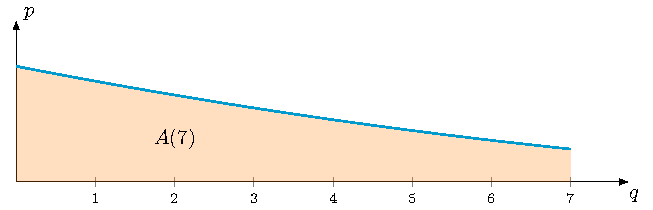
\includegraphics[width = 4.8cm, height = 3.5cm]{img/area-total-value.pdf}
    }
    \end{minipage}
    \begin{minipage}{0.475\textwidth}
        
        This problem of finding the TCV, when \textbf{infinitely many infinitesimal} batches are delivered and consumed continuously at the same pace, is solved by finding \textbf{the area under the demand curve}, which is an application of integral calculus. 
    \end{minipage}
    
\end{frame}

\begin{frame}{The area under a (positive) curve}

    Take a positive function, $f(x) > 0$, and its area from $x = 0$ to $x = t$, denoted by $A(t)$.
    \vspace{0.3cm}
    
    Note that $\frac{A(t+h) - A(t)}{h} \approx f(t)$ for $h\approx 0$. The approximation gets better as $h$ gets smaller. 
    \vspace{-0.3cm}
    
    \begin{align*}
        \text{Hence:}\quad A'(t) = \lim_{h\rightarrow 0} \frac{A(t+h) - A(t)}{h} = f(t)\quad (\text{That is, the derivative of } A \text{ is } f).
    \end{align*}
    
    \begin{center}
    \vspace{-0.3cm}
    
    $\Big\Downarrow$
    
    \textbf{Finding the area under $\pmb{f}$} is equivalent to \textbf{finding $\pmb{f}$'s ``anti-derivative''}.    
    \end{center}
    
    
    \begin{center}
        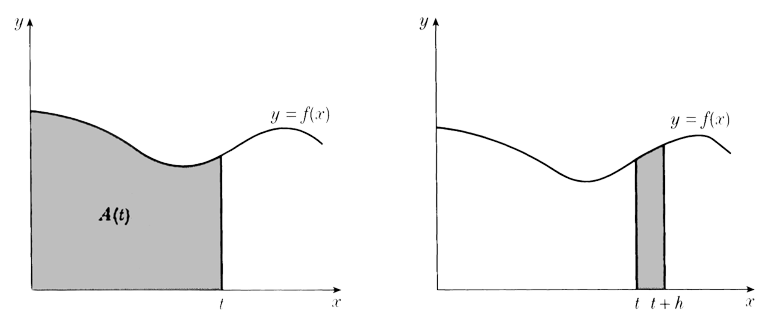
\includegraphics[width = 0.9\textwidth, height = 4cm]{img/area-increment.png}
    \end{center}
    
\end{frame}

\begin{frame}{``anti-derivatives'' and (indefinite) integrals}

    \begin{minipage}{0.63\textwidth}
        \begin{block}{Indefinite integrals definition}
        $F(x)$ is the (indefinite) integral of $f(x)$ if $F'(x) = f(x)$.
        \end{block}        
    \end{minipage}\hspace{0.3cm}
    \begin{minipage}{0.33\textwidth}
        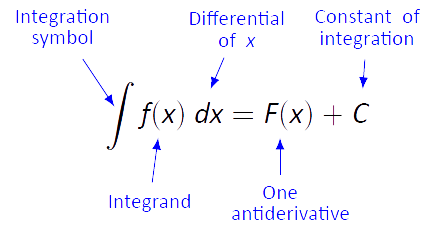
\includegraphics[width = \textwidth]{img/integral-notation.png}
    \end{minipage}
    \vspace{0cm}

    \begin{block}{Indefinite integrals are unique up to additive constants}
        If $F$ and $G$ are both indefinite integrals of $f$, then, for $H = F - G$,
        $$
        H'(x) = F'(x) - G'(x) = f(x) - f(x) = 0.
        $$
        That is, $H(x)$ is constant, meaning that $F(x) = G(x) + c$, for some (constant of integration) $c\in\R$.    
    \end{block}

    \begin{block}{(Dummy) variable of integration}
        The variable of integration (after the differential operator and in the integrand) is a dummy variable, meaning that it can be changed by any other variable:
        $$
        \int f(x)\,\rmd x = \int f(t)\,\rmd t.
        $$
    \end{block}

\end{frame}

\begin{frame}{Indefinite integrals. An example}

    \begin{block}{Example}
        Find the family of indefinite integrals of $f(x) = 2x$.

        We can check that, for any function $F_c(x) = x^2 + c$, with $c\in\R$, $F_c'(x) = f(x)$.
        \vspace{-0.3cm}
        
        $$
        \textbf{Notation: } \int 2x\,\rmd x = x^2 + c.
        $$ 
    \end{block}
    \vspace{0.2cm}

    \begin{center}
        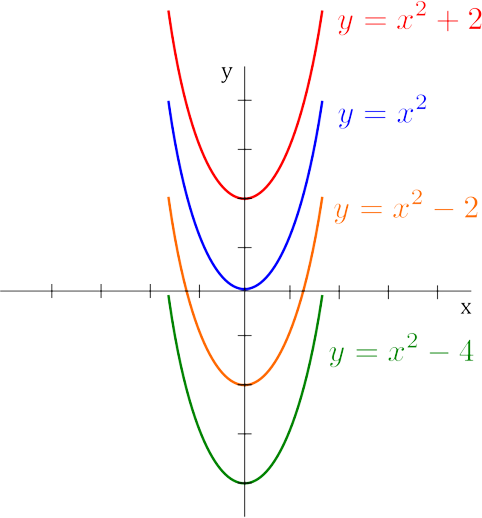
\includegraphics[width = 0.4\textwidth, height = 4cm]{img/integral-constant-x2.png}
    \end{center}
    
\end{frame}

\begin{frame}{Linearity of integrals}

    \begin{block}{The integral operator is linear}
        From the linearity of the differential operator, it follows the linearity of integrals:
        \begin{enumerate}[leftmargin = 0.5cm, label = $\bullet$, rightmargin = 0.2cm]
            \item $\int (f(x) + g(x))\rmd x = \int f(x)\rmd x + \int g(x)\rmd x$.
            \item $\int k f(x)\rmd x = k\int f(x)\rmd x$.
        \end{enumerate}
    \end{block}

    \begin{minipage}{0.5\textwidth}
        \begin{block}{Example}
        Find the family of indefinite integrals of $f(x) = x^2 + 2x$.
        \begin{align*}
            \int (x^2 + 2x)\,\rmd x &= \int x^2\,\rmd x + \int 2x\,\rmd x\\
            &= x^3/3 + x^2 + c.
        \end{align*}
        \end{block}
    \end{minipage}
    \begin{minipage}{0.45\textwidth}
        \begin{center}
        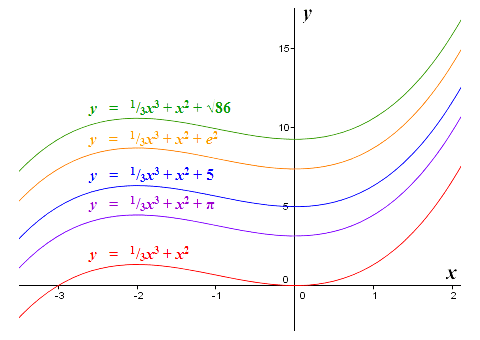
\includegraphics[width = 0.9\textwidth, height = 4cm]{img/integral-constant-unique.png}
        \end{center}    
    \end{minipage}

\end{frame}

\begin{frame}{Standard integrals}

    \begin{block}{Integral of standard functions}
        These are the integrals of some common functions
        \begin{enumerate}[leftmargin = 0.5cm, label = $\bullet$, rightmargin = 0.2cm]
            
            \item $\int x^a\rmd x = \frac{1}{a+1}x^{a+1} + c$, for $a\neq -1$

            \item $\int \frac{1}{x}\rmd x = \ln(|x|) + c$

            \item $\int e^{ax}\rmd x = \frac{1}{a}e^{ax} + c$, for $a\neq 0$

            \item $\int \sin(x)\rmd x = -\cos(x) + c$

            \item $\int \cos(x)\rmd x = \sin(x) + c$
            
        \end{enumerate}
        
    \end{block}
    
\end{frame}

\begin{frame}{Definite integrals and Fundamental Theorem of Calculus}

    \begin{block}{Definite integral definition  and Fundamental Theorem of Calculus}
        Let $F(x)$ be an indefinite integral of $f(x)$. The definite integral of $f(x)$ from $x = a$ to $x = b$, denoted $\int_a^bf(x)\rmd x$, is defined to be the value $F(b) - F(a)$. That is,
        $$
        \int_a^bf(x)\rmd x = F(b) - F(a).\quad \text{FTC}
        $$
        The value $F(b) - F(a)$ is commonly represented by $F(x)\big|_a^b$
    \end{block}

    \begin{block}{Example}
        $$
        \int_1^2t^2\rmd t = t^3/3\big|_1^2 = 2^3/3 - 1^3/3 = 7/3.
        $$
    \end{block}
            
\end{frame}

\begin{frame}{Definite integrals as areas under positive functions}

    For a function $f(x)$ that is positive between $x = a$ and $x = b$, $\int_a^bf(x)\rmd x$ is the value of the area under $f(x)$ (and above the $x$-axis) from $x = a$ to $x = b$.

    \begin{block}{Example}
        Compute the area under the curve of the line $f(x) = px + q$ between $x = a$ and $x = b$, for positive values of $p, q, a$, and $b$, such that $b > a$.
        \vspace{0.2cm}
        
        \begin{minipage}{0.65\textwidth}
        Since $p, q, a$, and $b$ are positive, the function $f(x)$ is positive between $x = a$ and $x = b$. Hence, the area we are looking for is the definite integral of $f(x)$ from $x = a$ to $x = b$
        \begin{align*}
            \int_a^b (px+q)\rmd x = (px^2/2 + qx)\bigg|_a^b = p(b^2 - a^2)/2 + q(b - a).
        \end{align*}
        \end{minipage}\hspace{0.2cm}
        \begin{minipage}{0.3\textwidth}
            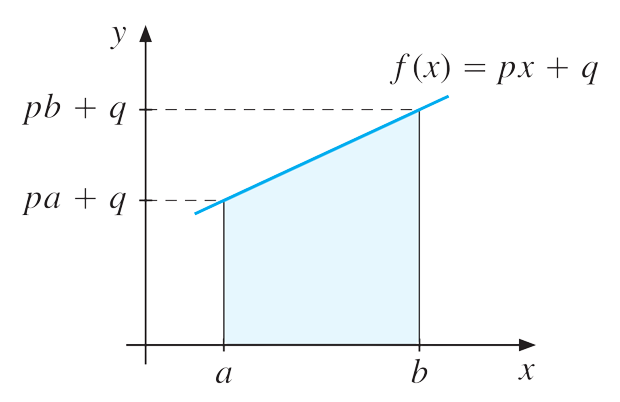
\includegraphics[width = \textwidth, height = 3cm]{img/area-under-line.png}
        \end{minipage}
    \end{block}

\end{frame}

\begin{frame}{Economic application. The consumer surplus.}

    We already introduced, as a motivating example, the notion of Total Consumption Value (TCV), that is, a function $TCV(x)$ such that
    \begin{align*}
        TCV(q) = \text{ Maximum amount consumers are willing to pay for } q \text{ items } = \int_0^q p_D(x)\, \rmd x,
    \end{align*}
    where $p_D$ is the (inverse) demand function.

    \begin{block}{Consumer Surplus}
        For a market with equilibrium quantity and price $q^*$ and $p^*$, respectively, the Consumer Surplus (CS) is defined as
        \begin{align*}
            CS &= \text{ The maximum amount consumers are willing to pay }\\
            &\hspace{0.45cm} \text{ minus what they would pay for buying } q^* \text{ units at } p^* \text{ dollars each } \\
            &= TCV(q^*) - q^*p^* = \int_0^{q^*} (p_D(q) - p^*)\,\rmd q.
        \end{align*}
        The CS can be interpreted as the amount of money consumers would save by buying all $q^*$ units at once at $p^*$ dollars each, vs buying continuously as producers deliver up to $q^*$ units of product.
    \end{block}
    
\end{frame}

\begin{frame}{The consumer surplus. An example}

    \begin{minipage}{0.5\textwidth}
        \begin{block}{Problem}
            The demand and supply set for a given product is given by
            \begin{align*}
                D &= \{(q, p) : q + 200p = 2600\}, \\
                S &= \{(q, p) : q - 100p = -1000\}.
            \end{align*}
            Compute the CS.
        \end{block}
    \end{minipage}
    \begin{minipage}{0.45\textwidth}
        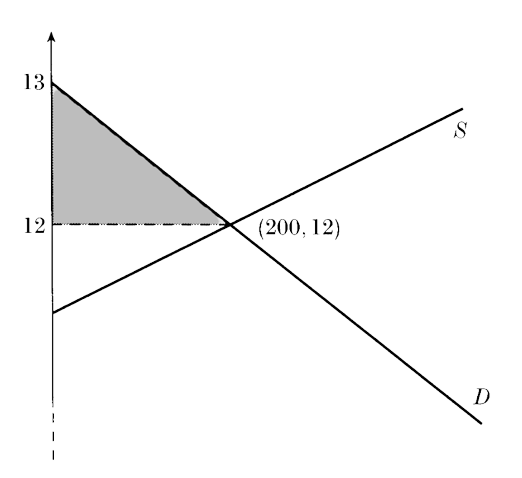
\includegraphics[width = \textwidth, height = 4cm]{img/CS.png}
    \end{minipage}
    \vspace{0.1cm}
    
        \textbf{Solution:} 
        \vspace{-0.2cm}
        \begin{enumerate}[leftmargin = 0.5cm, label = \arabic*., rightmargin = 0.2cm]
            \item Find the (inverse) demand function: $p_D(q) = 13 - q/200$.
            \item Compute the equilibrium price and quantity: $p^* = 12$ and $q^* = 200$. 
            \item Calculate the CS: 
            \begin{align*}
                \int_0^{q^*} p_D(q)\,\rmd q - q^*p^* &= \int_0^{200} (13 - q/200)\, \rmd q - 12*200 \\
                &= (13q - q^2/400)\big|_0^{200} - 2400 = 
                %(13\times 200 - 200^2/400)\big|_0^{200} = 
                %2600 - 100 - 2400 = 
                100 
            \end{align*}
        \end{enumerate}
    
\end{frame}

\begin{frame}{Economic application. Lorenz curves, the Gini Index and inequality.}

    \begin{block}{The Lorenz curve}
    The \textbf{Lorenz curve} $L(x)$, developed by the economist Max Lorenz in 1905, represents inequality of the wealth distribution.
    \begin{align*}
        L(x) = \text{ proportion of overall wealth held by the bottom } x\% \text{ of the people}. 
    \end{align*}
    \textbf{Example:} $L(0.5) = 0.2 \Rightarrow$ the poorest $50\%$ of the population holds $20\%$ of the wealth.
    \end{block}

    \begin{minipage}{0.58\textwidth}
        \begin{center}
            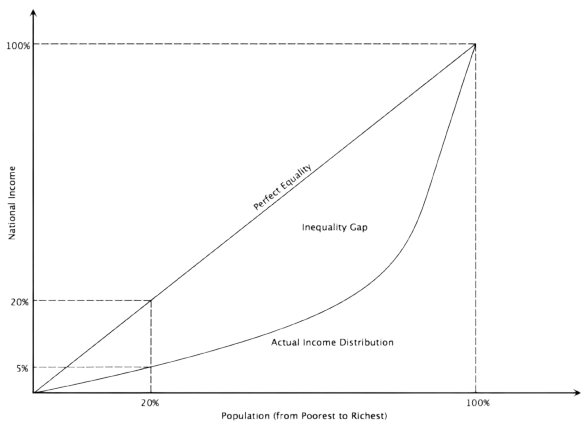
\includegraphics[width = 6cm, height = 4cm]{img/Lorenz.png}    
        \end{center}    
    \end{minipage}
    \begin{minipage}{0.4\textwidth}
        The Lorenz curve must satisfy
        \begin{enumerate}[leftmargin = 0.4cm, label = $\bullet$, rightmargin = 0.2cm]
            \item $L(0) = 0$ and $L(1) = 1$
            \item $L$ is non-decreasing
            \item $L(x) \leq x$
        \end{enumerate}
    \end{minipage}
    
\end{frame}

\begin{frame}{Economic application. Lorenz curves, the Gini Index and inequality.}

    \begin{block}{Gini Index (GI)}
        The Gini coefficient was proposed by the statistician  Corrado Gini in 1912, as a measure of inequality of wealth distribution.

        The idea is to measure how the Lorenz curve (representing wealth distribution) departs from the $PE(x) = x$ curve (representing perfect equality).

        \textbf{Definition of GI:} $GI = A/(A+B)$, where:
        \vspace{-0.2cm}
        
        \begin{enumerate}[leftmargin = 0.2cm, label = , rightmargin = 0.2cm]
            \item $\pmb{A}$\textbf{:} area between the Lorenz curve and the perfect equality curve, 
            \item $\pmb{B}$\textbf{:} area under the Lorenz curve.
        \end{enumerate}
        
    \end{block}

    % \begin{minipage}{0.45\textwidth}
    \begin{center}
        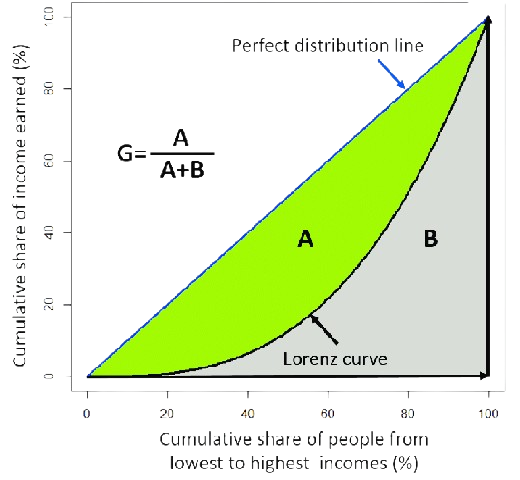
\includegraphics[width = 6cm, height = 3cm]{img/Lorenz-curve-and-Gini-coefficient.png}
    \end{center}
    % \end{minipage}
    
\end{frame}

\begin{frame}{Lorenz curves, the Gini Index and inequality. An example.}

    \begin{minipage}{0.5\textwidth}
        \begin{block}{Problem}
            \begin{enumerate}[leftmargin = 0.5cm, label = \arabic*., rightmargin = 0.2cm]
            \item Show that $0 \leq GI \leq 1$
            \item Show that $GI = 2\int_0^1 (x - L(x))\,\rmd x$
            \item What is $L(x)$ when $GI = 0$ and $GI = 1$?
            \item Calculate the Gini index for: 
            \begin{enumerate}[leftmargin = 0.5cm, label = (\alph*), rightmargin = 0.2cm]
                \item $L(x) = x^4$
                \item $L(x) = \frac{1}{3} x^3 + \frac{2}{3} x^5$
            \end{enumerate}
        \end{enumerate}
        \end{block}
    \end{minipage}
    \begin{minipage}{0.45\textwidth}
        \quad \textbf{Solution:}
    \end{minipage}
    \vspace{0.1cm}

        \begin{center}
            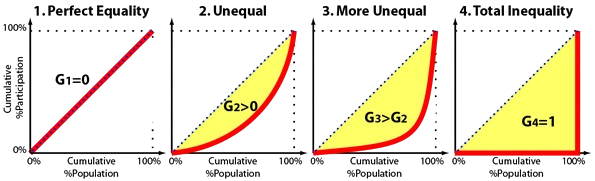
\includegraphics[width = \textwidth, height = 4cm]{img/gini_sorted.png}
        \end{center}
    
\end{frame}

\begin{frame}{Properties of definite integrals}

    \begin{block}{Properties of definite integrals}
        These properties are easy to obtain from the definition of definite integral
        \begin{enumerate}[leftmargin = 0.5cm, label = $\bullet$, rightmargin = 0.2cm]
            \item $\int_a^bf(x)\rmd x = \int_a^c f(x)\rmd x + \int_c^bf(x)\rmd x$, for $a < c < b$.

            \item $\int_a^a f(x)\rmd x = 0$.

            \item $\int_a^b f(x)\rmd x = -\int_b^af(x)\rmd x$.

            \item $\int_a^b (f(x) + g(x))\rmd x = \int_a^b f(x)\rmd x + \int_a^b g(x)\rmd x$.

            \item $\int_a^b kf(x)\rmd x = k\int_a^b f(x)\rmd x$, $k\in\R$.

            \item If $f(x) \leq g(x)$ for all $x\in (a, b)$, then $\int_a^b f(x)\,\rmd x \leq \int_a^b g(x)\,\rmd x$.
        \end{enumerate}        
    \end{block}

\end{frame}

\begin{frame}{Application of the properties of integrals: \\ Areas above negative functions}

    \textbf{Property:} $\int_a^b kf(x)\rmd x = k\int_a^b f(x)\rmd x$, $k\in\R$.
    
    \textbf{Use:} For a function $f(x)$ that is negative between $x = a$ and $x = b$, $\int_a^bf(x)\rmd x$ is minus the value of the area above $f(x)$ (and under the $x$-axis) from $x = a$ to $x = b$.

    \begin{block}{Example}
        Compute the area under the curve of the function $f(x) = e^{x/3} - 3$ from $x = 0$, to $x = 3\ln(3)$.
        \vspace{0.2cm}
        
        \begin{minipage}{0.65\textwidth}
        Since $e^{x/3} - 3$ is negative between $x = 0$ and $x = 3\ln(3)$, the area we are looking for is minus the definite integral of $f(x)$ from $x = 0$ to $x = 3\ln(3)$.
        \begin{align*}
            -\int_0^{3\ln(3)} (e^{x/3} - 3)\rmd x &= -(3e^{x/3} - 3x)\bigg|_0^{3\ln(3)} \\
            &= -((9 - 9\ln(3)) - 3) \\
            &= 3(3\ln(3) - 2).
        \end{align*}
        \end{minipage}\hspace{0.2cm}
        \begin{minipage}{0.3\textwidth}
            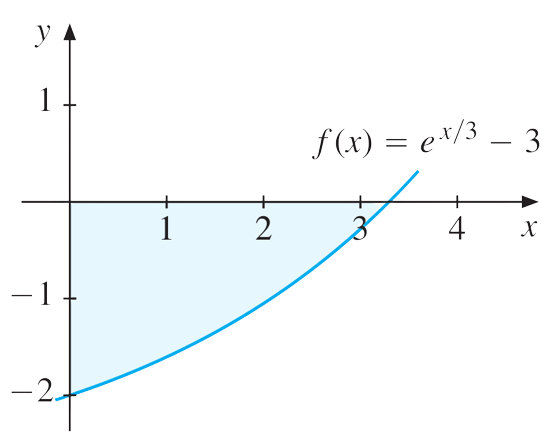
\includegraphics[width = \textwidth, height = 3cm]{img/area-under-exp.png}
        \end{minipage}
    \end{block}
    
\end{frame}

\begin{frame}{Definite integrals as areas delimited by functions changing signs}

    \begin{minipage}{0.51\textwidth}
        Using the interpretation of definite integrals as areas delimited by positive and negative functions, we can compute the area delimited by functions that change signs.
    \end{minipage}\hspace{0.2cm}
    \begin{minipage}{0.43\textwidth}
        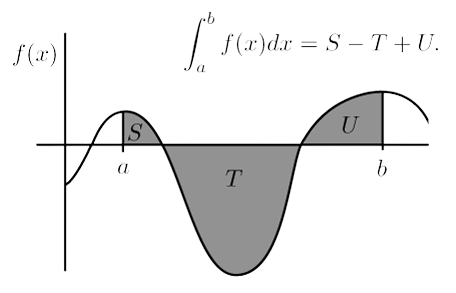
\includegraphics[width = \textwidth, height = 2.2cm]{img/area-positive-negative.png}
    \end{minipage}

    
    \begin{block}{Example}
        Compute the area under the curve of the function $f(x) = \sin(x)$ from $x = 0$, to $x = 2\pi$.
        \vspace{0.2cm}
        
        \begin{minipage}{0.65\textwidth}
        Since $\sin(x)$ is positive between $x = 0$ and $x = \pi$, and negative between $x = \pi$ and $x = 2\pi$, the area we are looking for is
        \begin{align*}
            &\int_0^\pi \sin(x)\rmd x - \int_\pi^{2\pi} \sin(x)\rmd x \\
            &= -\cos(x)\bigg|_0^\pi + \cos(x)\bigg|_\pi^{2\pi} \\
            &= (-\cos(\pi) + \cos(0)) + (\cos(2\pi) - \cos(\pi)) = 4
        \end{align*}
        \end{minipage}\hspace{0.2cm}
        \begin{minipage}{0.3\textwidth}
            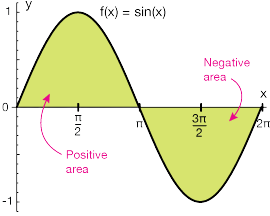
\includegraphics[width = \textwidth, height = 3cm]{img/area-sin.png}
        \end{minipage}
    \end{block}
    
\end{frame}

\begin{frame}{Application of the properties of integrals: \\ Areas delimited by piecewise-defined functions}

    \textbf{Property:} $\int_a^bf(x)\rmd x = \int_a^c f(x)\rmd x + \int_c^bf(x)\rmd x$, for $a < c < b$

    \begin{minipage}{0.45\textwidth}
        \begin{block}{Problem}
        Find the area enclosed by the curve $h(x) = \min(f(x), g(x))$, with $f(x) = x^3$, $g(x) = 1/x^2$, the $x$-axis, and the lines $x = 1/2$ and $x = 2$.
        \end{block}    
    \end{minipage}\hspace{0.3cm}
    \begin{minipage}{0.45\textwidth}
        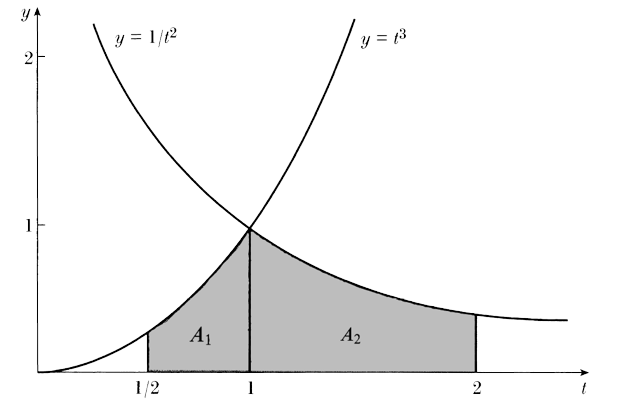
\includegraphics[width =  \textwidth, height = 3cm]{img/area-many-functions.png}
    \end{minipage}

    \textbf{Solution:} Note that the upper bound of the area in hand is given by $f(x)$, for $x = (1/2, x^*)$, and by $g(x)$, from $x = (x^*, 2)$, where $x^*$ is the $x$-coordinate of the point of intersection of $f(x)$ and $g(x)$, that is,
    \begin{align*}
        f(x^*) = g(x^*)\, \Longleftrightarrow x^* = 1.
    \end{align*}
    Therefore, being $A$ the area to be computed,
    \begin{align*}
        A &= \int_{1/2}^1 f(x)\,\rmd x + \int_1^2 g(x)\,\rmd x = x^4/4\big|_{1/2}^1 -1/x\big|_1^2 
        = \frac{1}{4} - \frac{1}{64} - \lrp{\frac{1}{2} - 1} = \frac{47}{64}
    \end{align*}
    
\end{frame}


%----------------------- INTRODUCTION TO INTEGRAL CALCULUS -----------------------%


\section{Integration techniques}
%----------------------- TECHNIQUES OF INTEGRATION -----------------------%
\begin{frame}{Integration techniques}

    \textbf{Why do we need integration techniques?}
    \begin{enumerate}[leftmargin = 0.5cm, label = $\bullet$, rightmargin = 0.2cm]

    \item Unlike computing derivatives, \textbf{finding integrals may be very challenging.}
    \vspace{0.2cm}

    \item So far, we have been guessing rather than computing integrals.
    \vspace{0.2cm}

    \item It is easy to guess a function whose derivative is $f(x) = x^2$.
    \vspace{0.2cm}

    \item But it is not that easy to make the guess for $f(x) = x\sqrt{3x^2 + 5}$.
    \vspace{0.2cm}

    \item We need \textbf{integration techniques to address these harder integrals}, by reducing them to simpler integrals that can be solved by the guess-and-verify method

    \end{enumerate}
    
\end{frame}

\begin{frame}{Integration techniques. Understanding versus computing.}
\small

    \textbf{Computing versus understanding integrals}
    \begin{enumerate}[leftmargin = 0.5cm, label = $\bullet$, rightmargin = 0.2cm]

    \item This course does not focus on computing integrals, but understanding them.
    \vspace{0.2cm}

    \item Applications of integrals are what matters (Gini index, consumer surplus, etc).
    \vspace{0.2cm}

    \item For handling complicated integrands, you may rely on software (Maple, Methematica, etc).
    \vspace{0.2cm}

    \item AI tools may also come in handy, but watch out for hallucinations.
    \end{enumerate}

    \textbf{Basic integration techniques}
    \begin{enumerate}[leftmargin=0.5cm,label=$\bullet$]
      \item Substitution (a.k.a change of variable) (reverse chain rule) \\
      \textit{Pattern:} $\displaystyle \int f(g(x))\,g'(x)\,\rmd x \;\to\; u=g(x),\; \rmd u=g'(x)\,\rmd x,\; \int f(u)\,\rmd u$.\\
      \emph{When it helps:} the substitution turns the integrand into a simpler, standard form.\\
      \emph{Example:} $\displaystyle \int x\sqrt{3x^2+5}\,\rmd x \xrightarrow{u=3x^2+5} \int \tfrac{1}{6}u^{1/2}\,\rmd u = \tfrac{(3x^2+5)^{3/2}}{9}+C$.
    
      \item Integration by parts (reverse product rule) 
      \item Partial fractions (decompose rational functions to sum of simples.
.\end{enumerate}
    
\end{frame}


%----------------------- TECHNIQUES OF INTEGRATION -----------------------%

%----------------------- IMPROPER INTEGRALS -----------------------%
\section{Improper integrals}

\begin{frame}{Improper integrals with infinite intervals of integration}

    Many economic and statistical applications use the concept of integrals over an infinite integration interval.

    \begin{block}{(Improper) integrals and infinite intervals of integration}
    For a function $f(x)$ and a constant $a\in\R$,
        \begin{align*}
            \int_a^\infty f(x)\rmd x &:= \lim_{y\rightarrow \infty} \int_a^y f(x)\,\rmd x,\quad
            \int_{-\infty}^a f(x)\rmd x := \lim_{y\rightarrow -\infty} \int_y^a f(x)\,\rmd x.
        \end{align*}
    If the limits above converge, the associated integrals are said to converge. Otherwise, they diverge. For both limits of integration being infinite,
    \begin{align*}
            \int_{-\infty}^\infty f(x)\rmd x &:= \int_{-\infty}^a f(x)\rmd x + \int_a^\infty f(x)\rmd x.
    \end{align*}
    If both integrals on the right hand converge, the integral on the left hand is said to converge.
    \end{block}

\end{frame}

\begin{frame}{Improper integrals with infinite integration intervals. An example}

    \begin{minipage}{0.56\textwidth}
        The exponential distribution is used in Probability Theory to represent randomness in waiting times and decay/growth processes.
        \vspace{0cm}
        \begin{block}{Example. The exponential distribution}
        
        Compute the integral $\int_0^\infty \lambda e^{-\lambda x}\,\rmd x$, for $\lambda > 0$.
        \begin{align*}
            \int_0^\infty \lambda e^{-\lambda x}\,\rmd x &= \lim_{t\rightarrow\infty}\lambda\int_0^t e^{-\lambda x}\,\rmd x \\
            &= \lim_{t\rightarrow\infty} (1 - e^{-\lambda t}) = 1.
        \end{align*}
        \end{block}
        \vspace{0cm}
        
        The area $A$ has an unbounded base, but the height decreases to $0$ so fast that the area is $1$.
    \end{minipage}\hspace{0.28cm}
    \begin{minipage}{0.4\textwidth}
        \vspace{-0.2cm}
        
        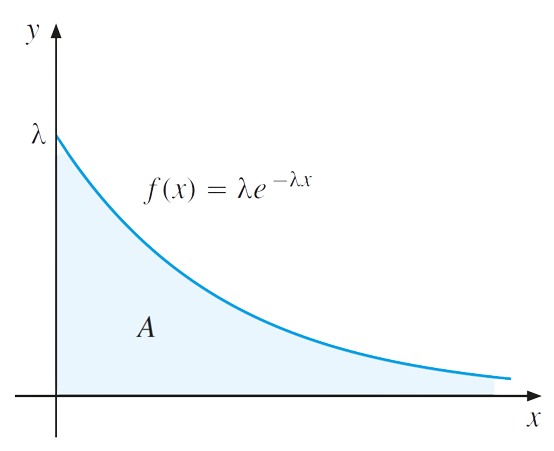
\includegraphics[width = 5cm, height = 5.7cm]{img/improper-int-exp.png}
    \end{minipage}
\end{frame}

\begin{frame}{Improper integrals of unbounded functions}

    The other type of improper integral is when the integrand is not bounded.

    \begin{block}{(Improper) integrals of unbounded functions}
    For a function \(f\) defined on \(\blue{(a,b]}\) (resp. \(\orange{[a,b)}\)) and not necessarily defined at \(\blue{x=a}\) (resp. \(\orange{x=b}\)),
    \[
    \blue{\int_a^b f(x)\,dx := \lim_{h\to0^+}\int_{a+h}^b f(x)\,dx},\quad
    \orange{\int_a^b f(x)\,dx := \lim_{h\to0^+}\int_a^{b-h} f(x)\,dx}.
    \]
    If the limits above converge, the associated integrals are said to converge. Otherwise, they diverge.
    \medskip
    
    If $f(x)$ is defined in $(a, b)$ but not necessarily at both boundary points $x = a$ and $x = b$, then, for any $c\in(a, b)$,
    \begin{align*}
        \int_a^b f(x)\rmd x &:= \int_a^c f(x)\rmd x + \int_c^b f(x)\rmd x.
    \end{align*}
    If both integrals on the right hand converge, the integral on the left hand is said to converge.
    \end{block}

\end{frame}

\begin{frame}{Improper integrals of unbounded functions. An Example}

    \begin{minipage}{0.56\textwidth}
        \begin{block}{Example.}
        Compute $\int_0^2\frac{1}{\sqrt{x}}\,\rmd x$.
        \begin{align*}
            \int_0^2 \frac{1}{\sqrt{x}}\,\rmd x &= \lim_{h\rightarrow 0^+}\int_h^2 \frac{1}{\sqrt{x}}\,\rmd x \\
            &= \lim_{h\rightarrow 0^+} 2(\sqrt{2} - \sqrt{h}) = 2\sqrt{2}.
        \end{align*}
        \end{block}
        \vspace{0cm}
    
        The area has an unbounded height for $x\rightarrow 0^+$, but the base decreases to $0$ so fast that the area is finite.
    \end{minipage}\hspace{0.28cm}
    \begin{minipage}{0.4\textwidth}
        \vspace{-0.2cm}

        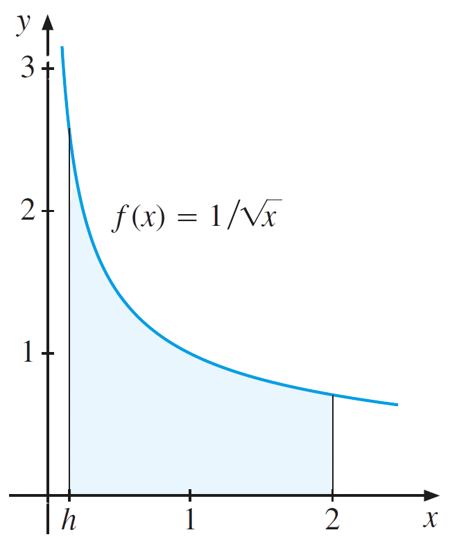
\includegraphics[width = 5cm, height = 5.7cm]{img/improper-int-invsqrt.png}
        
    \end{minipage}
    
\end{frame}

\begin{frame}{Comparison test for convergence of improper integrals}

    Recall the comparison property of definite integrals:
    \begin{align*}
        f(x) \leq g(x) \text{ for all } x\in (a, b) \Longrightarrow \int_a^b f(x)\,\rmd x \leq \int_a^b g(x)\,\rmd x.
    \end{align*}
    From this, we can obtain the following comparison test to get the convergence of an improper integral

    \begin{block}{Comparison test for convergence}
        Let $f$ and $g$ be functions defined in $(a, b)$, where $a$ and $b$ might be infinite or points where both functions are not defined. Assume that $|f(x)| \leq g(x)$ for all $x\in(a, b)$. Then
        \begin{align*}
            \int_a^b g(x)\,\rmd x < \infty \Longrightarrow \int_a^b f(x)\,\rmd x\  \text{ converges},
        \end{align*}
        and
        \begin{align*}
            \left|\int_a^b f(x)\,\rmd x\right| \leq \int_a^b g(x)\,\rmd x.
        \end{align*}
    \end{block}
    
\end{frame}

\begin{frame}{Comparison test. An example}

    One of the most important functions in Probability Theory and Statistics is the Gaussian (or bell-shaped) function, that is, $f(x) = e^{-x^2}$.

    

    \begin{minipage}{0.6\textwidth}
        The convergence of the integral $\int_{-\infty}^{\infty} e^{-x^2}\,\rmd x$ cannot be checked by means of the definition, as $f(x)$ is not integrable in terms of elementary functions (that is, its integral over a finite interval exists but is not a composition of standard functions)
    \end{minipage}
    \begin{minipage}{0.35\textwidth}
        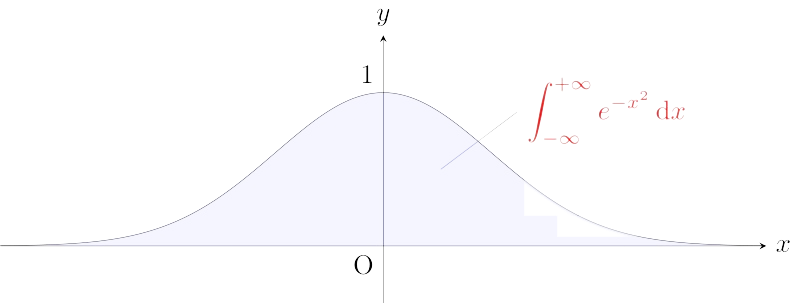
\includegraphics[width = \textwidth, height = 3cm]{img/gaussian-int.png}
    \end{minipage}

    \begin{block}{Example. Convergence of the Gaussian function}
        Proof that $\int_{-\infty}^{\infty} e^{-x^2}\,\rmd x$ converges.
        \begin{align*}
            \int_{-\infty}^{\infty} e^{-x^2}\,\rmd x &= 2\int_{0}^{\infty} e^{-x^2}\,\rmd x
            = 2\left(\int_{0}^{1} e^{-x^2}\,\rmd x + \int_{1}^{\infty} e^{-x^2}\,\rmd x\right) \\
            &\leq 2\left(\int_{0}^{1} \,\rmd x + \int_{1}^{\infty} e^{-x}\,\rmd x\right) \\
            &= 2(1 + \lim_{a\rightarrow\infty}(e^{-1} - e^{-a}))
            = 2(1 + e^{-1}) 
        \end{align*}
    \end{block}
    
    
\end{frame}
%----------------------- IMPROPER INTEGRALS -----------------------%

\end{document}
